\subsection{Basic Rules}\label{subsec:basic-rules}

\begin{enumerate}
    \item FTC: $F(b)=F(a)+\int_{a}^{b}f(x)dx$
    \item Power rule: $\int{x^n}dx=\frac{x^{n+1}}{n+1}$
\end{enumerate}

\subsubsection{U-Substitution}

\begin{gather*}
    \int_{2}^{5}x(3x^2)dx \Rightarrow u=3x^2, du=6xdx\\
    \Rightarrow \frac{1}{6}\int_{12}^{75}udu\\
    \frac{1}{6}[\frac{u^2}{2}|_{75}-\frac{u^2}{2}|_{12}]\\
\end{gather*}

\subsubsection{Integration by Partial Fractions}

Factor denominator, separate into partial fractions, then integrate.

\begin{gather*}
    \int{\frac{1}{x^2-4}}dx \Rightarrow \frac{1}{x^2-4}=\frac{1}{(x+2)(x-2)}\\
    \frac{1}{(x+2)(x-2)} \Rightarrow \frac{A}{x+2}+\frac{B}{x-2} \Rightarrow A=-\frac{1}{4}, B=\frac{1}{4}\\
    \int{\frac{-\frac{1}{4}}{x+2}+\frac{\frac{1}{4}}{x-2}}dx=-\frac{1}{4}\ln{|x+2|}+\frac{1}{4}\ln{|x-2|}+C\\
\end{gather*}

\subsubsection{Trigonometric Integrals}

Trigonometric Integrals
\begin{itemize}
    \item $\int{\sin{x}}\:dx=-\cos{x}+C$
    \item $\int{\cos{x}}\:dx=\sin{x}+C$
    \item $\int{\tan{x}}\:dx=-\ln{\cos{x}}+C$
    \item $\int{\cot{x}}\:dx=\ln{\sin{x}}+C$
    \item $\int{\sec{x}}\:dx=\ln{(\sec{x}+\tan{x})}+C$
    \item $\int{\csc{x}}\:dx=\ln{(\csc{x}-\cot{x})}+C$
    \item $\int{\sec{x}\tan{x}}\:dx=\sec{x}+C$
    \item $\int{-\csc{x}\cot{x}}\:dx=\csc{x}+C$
    \item $\int{\sec^2{x}}\:dx=\tan{x}+C$
    \item $\int{-\csc^2{x}}\:dx=\cot{x}+C$
\end{itemize}
Inverse Trigonometric Integrals
\begin{itemize}
    \item $\int{\frac{dx}{f(x)^2+a^2}}=\frac{1}{a}\arctan{\frac{f(x)}{a}}+C$
    \item $\int{\frac{dx}{\sqrt{a^2-f(x)^2}}}=\arcsin{\frac{f(x)}{a}}+C$
\end{itemize}

\subsection{Properties of Integrals}\label{subsec:properties-of-integrals}

\begin{enumerate}
    \item $\int_{a}^{a}f(x)dx=0$
    \item If $f(x)$ is odd, $\int_{-a}^{a}f(x)dx=0$
    \item If $f(x)$ is even and $\int_{0}^{a}f(x)dx=k$, then $\int_{-a}^{a}f(x)dx=2k$
    \item $\int_{a}^{b}f(x)dx+\int_{b}^{c}f(x)dx=\int_{a}^{c}f(x)dx$
    \item If $\int_{a}^{b}f(x)dx=k$, then $\int_{b}^{a}f(x)dx=-k$
    \item If $f(x) \leq g(x)$ $\forall x \in [a,b]$ then $\int_{a}^{b}f(x)dx \leq \int_{a}^{b}g(x)dx$
    \item $\vert \int_{a}^{b}f(x)dx \vert \leq \int_{a}^{b}|f(x)|dx$
\end{enumerate}

\subsection{Riemann Sums}\label{subsec:riemann-sums}

\subsubsection{Riemann Sum Notation and Definite Integrals}

\[\lim_{n\to{\infty}}\sum_{k=1}^{n}f(a+k\Delta{x})\Delta{x}\]

In $\Delta{x}=\frac{b-a}{n}$ (the subintervals), $b$ is the end limit of the integral which is the same as 
$a+n\Delta{x}$.
This can be used to solve for $b$ given $a$. $x$ can be represented
as $a+k\Delta{x}$.

\[\int_{a}^{b}f(x)dx=\lim_{n\to\infty}\sum_{k=1}^{n}f(a+\frac{k(b-a)}{n})\frac{b-a}{n}\]

\subsubsection{Basic Riemann Sums}

Left sum: $(x_R-x_L)f(x_L)$

\bigskip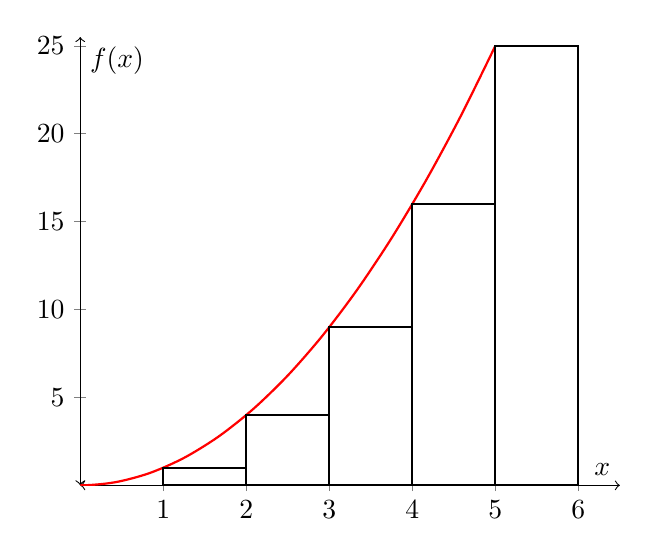
\begin{tikzpicture}
    \begin{axis}[
        xmin=0,xmax=6.5,
        ymin=0,ymax=25.5,
        axis x line=middle,
        axis y line=middle,
        axis line style=<->,
        xlabel={$x$},
        ylabel={$f(x)$}
        ]
    \addplot[red,thick,smooth] {x^2};
    \draw[draw=black,thick] (1,0) rectangle (2,1);
    \draw[draw=black,thick] (2,0) rectangle (3,4);
    \draw[draw=black,thick] (3,0) rectangle (4,9);
    \draw[draw=black,thick] (4,0) rectangle (5,16);
    \draw[draw=black,thick] (5,0) rectangle (6,25);
    \end{axis}
\end{tikzpicture}\bigskip

Right sum: $(x_R-x_L)f(x_R)$

\bigskip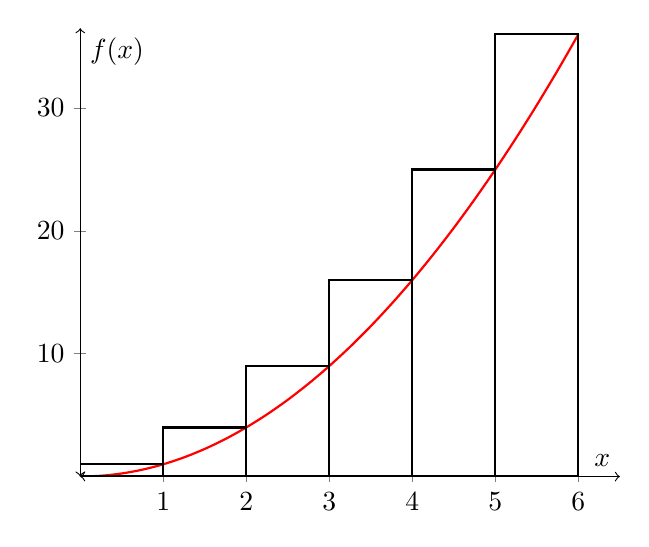
\begin{tikzpicture}
    \begin{axis}[
        xmin=0,xmax=6.5,
        ymin=0,ymax=36.5,
        axis x line=middle,
        axis y line=middle,
        axis line style=<->,
        xlabel={$x$},
        ylabel={$f(x)$}
        ]
    \addplot[red,thick,smooth,domain=0:6] {x^2};
    \draw[draw=black,thick] (0,0) rectangle (1,1);
    \draw[draw=black,thick] (1,0) rectangle (2,4);
    \draw[draw=black,thick] (2,0) rectangle (3,9);
    \draw[draw=black,thick] (3,0) rectangle (4,16);
    \draw[draw=black,thick] (4,0) rectangle (5,25);
    \draw[draw=black,thick] (5,0) rectangle (6,36);
    \end{axis}
\end{tikzpicture}\bigskip

Midpoint sum: $(x_R-x_L)f(x_L+\frac{x_R-x_L}{2})$

\bigskip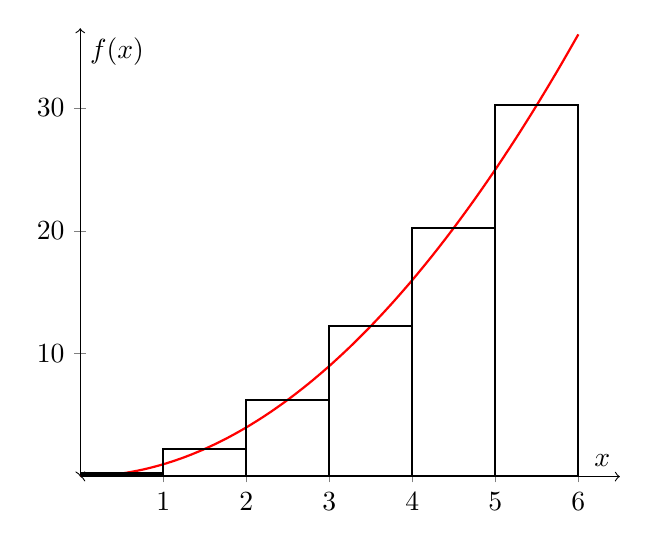
\begin{tikzpicture}
    \begin{axis}[
        xmin=0,xmax=6.5,
        ymin=0,ymax=36.5,
        axis x line=middle,
        axis y line=middle,
        axis line style=<->,
        xlabel={$x$},
        ylabel={$f(x)$}
        ]
    \addplot[red,thick,smooth,domain=0:6] {x^2};
    \draw[draw=black,thick] (0,0) rectangle (1,0.25);
    \draw[draw=black,thick] (1,0) rectangle (2,2.25);
    \draw[draw=black,thick] (2,0) rectangle (3,6.25);
    \draw[draw=black,thick] (3,0) rectangle (4,12.25);
    \draw[draw=black,thick] (4,0) rectangle (5,20.25);
    \draw[draw=black,thick] (5,0) rectangle (6,30.25);
    \end{axis}
\end{tikzpicture}\bigskip

Trapezoidal sum: $\frac{1}{2}(f(x_R)+f(x_L))(x_R-x_L)$

\bigskip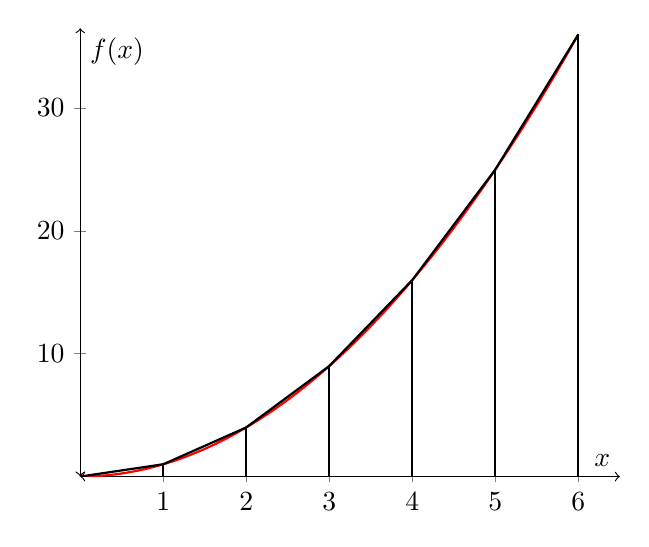
\begin{tikzpicture}
    \begin{axis}[
        xmin=0,xmax=6.5,
        ymin=0,ymax=36.5,
        axis x line=middle,
        axis y line=middle,
        axis line style=<->,
        xlabel={$x$},
        ylabel={$f(x)$}
        ]
    \addplot[red,thick,smooth,domain=0:6] {x^2};
    \draw[black,thick] (0,0)--(1,1);
    \draw[black,thick] (1,1)--(1,0);
    \draw[black,thick] (1,1)--(2,4);
    \draw[black,thick] (2,4)--(2,0);
    \draw[black,thick] (2,4)--(3,9);
    \draw[black,thick] (3,9)--(3,0);
    \draw[black,thick] (3,9)--(4,16);
    \draw[black,thick] (4,16)--(4,0);
    \draw[black,thick] (4,16)--(5,25);
    \draw[black,thick] (5,25)--(5,0);
    \draw[black,thick] (5,25)--(6,36);
    \draw[black,thick] (6,36)--(6,0);
    \end{axis}
\end{tikzpicture}

\subsection{Integration by Parts}\label{subsec:integration-by-parts}

\[\int{f'(x)g(x)}dx=f(x)g(x)-\int{g'(x)f(x)}dx\]

Choose $g(x)$ in order of \textbf{logs, inverse, algebraic, trig, exponential}.

\subsubsection{Example}

\begin{gather*}
    \int{x\sqrt{x+1}}dx \Rightarrow g(x)=x, f'(x)=\sqrt{x+1}\\
    =\frac{x}{2}(x+1)^{3/2}-\int{\frac{1}{2}(x+1)^{3/2}}dx\\
    =\frac{x}{2}(x+1)^{3/2}-\frac{1}{5}(x+1)^{5/2}+C\\
\end{gather*}

\subsubsection{Tabular Method}

Negate every second entry under derivative column.

\[\int{x^2\sin{x}}\:dx \Rightarrow f(x)=x^2,\;g(x)=\sin{x}\]

\begin{center}
    \begin{tabular}{|c|c|}
        \hline
        $f(x)$ & $g(x)$\\
        \hline
        $x^2$ & $\sin{x}$\\
        \hline
        $-2x$ & $-\cos{x}$\\
        \hline
        $2$ & $-\sin{x}$\\
        \hline
        $0$ & $\cos{x}$\\
        \hline
    \end{tabular}
\end{center}

\[\int{x^2\sin{x}}\:dx=-x^2\cos{x}-2x\sin{x}+2\cos{x}+C\]